For one dimensional data, the evaluation covers the following tasks:

\begin{itemize}
	\item Find a structure for recursive model index empirically.
	\item Compares the performance between baseline model, recursive model and traditional B-Tree.
\end{itemize}

\subsection{Dataset}

For one dimensional case, we manually generate two columns of the data:

\begin{itemize}
	\item The first column contains the keys $X$, which is randomly sampled from a given distribution.
	\item Then we assign the keys into different pages according to a preset parameter $N_{page}$ for page size. Specifically, the first $N_{page}$ keys will be assigned into the first page, the second $N_{page}$ keys will be assigned into the second page and so on so forth. After the assignments, we set the second column $Y$ to be the page index of the corresponding $x$.
\end{itemize}

%%TODO: change this to a graph with multiple distributions

\begin{figure}[htp]
    \centering
    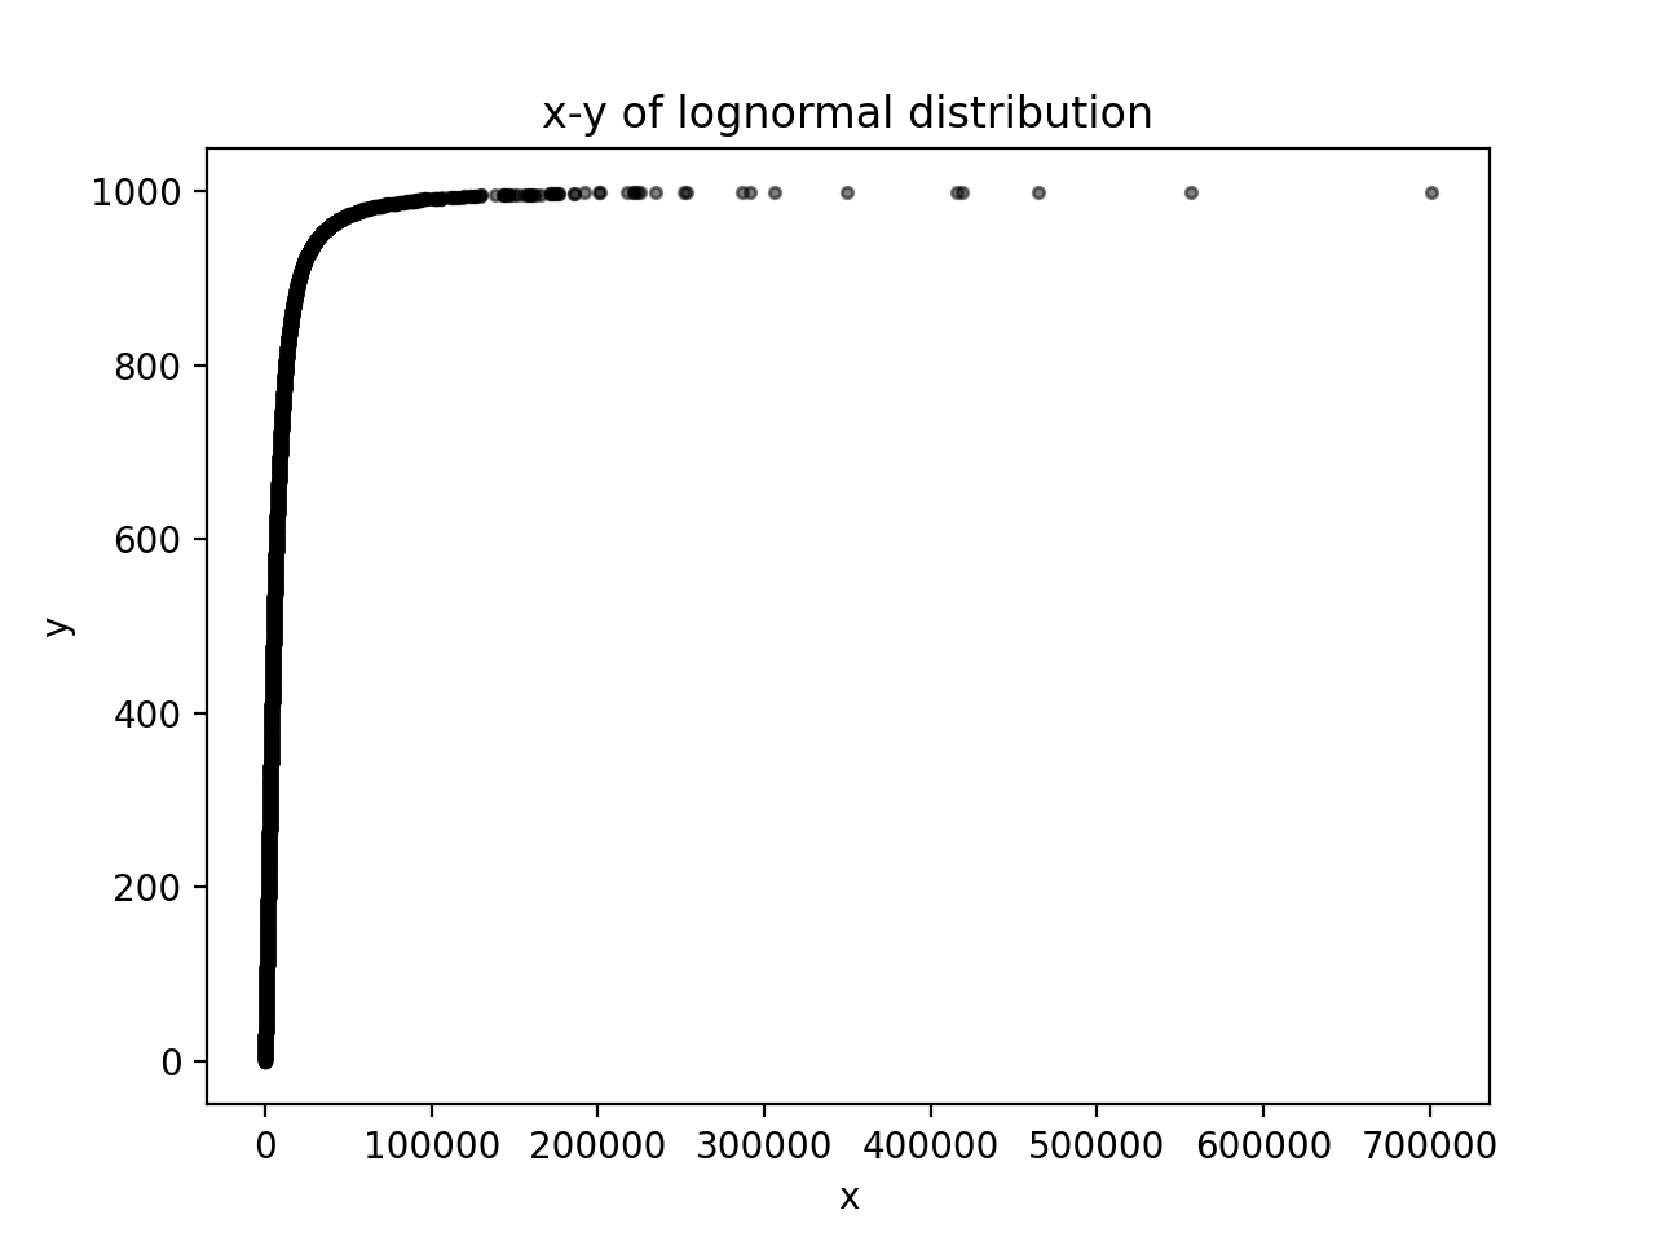
\includegraphics[width=0.6\textwidth]{graphs/evaluation/lognormal_distribution_x_y.pdf}
    \caption{The x-y graph where x is randomly sampled from a lognormal distribution}
    \label{fig:lognormal_x_y}
\end{figure}

\textbf{Small Lognormal Distributed Data} We first generate $10,000$ data points where $X$ is from a lognormal distribution $\text{Lognormal}(0, 4)$. In the Fig \ref{fig:lognormal_x_y}, we illustrate the $x-y$ relations where $X$ is randomly sampled from a lognormal distribution.



We use three groups to find the best recursive model for lognormal data.
\begin{itemize}
	\item All models are fully connected neural networks. The number of second-level models are $200, 400,$ and $600$ respectively. The number of third-level models are $2000, 4000$ and $6000$ for each number of second-level models.
	\item All models are linear regression models. The number of second-level models are $200, 400,$ and $600$ respectively. The number of third-level models are $2000, 4000$ and $6000$ for each number of second-level models.
	\item Models are combinations of fully connected neural networks and linear regression models. The numbers of second-level and third-level models are determined by the best settings in previous two group.
\end{itemize}

\begin{tikzpicture}[font=\small]
	\pgfplotsset{%
		width=0.55\textwidth,
		height=0.60\textwidth,
		minor grid style = {dotted},
	}
	\tikzstyle{every node}=[font=\footnotesize]
	\begin{groupplot}[group style={
                  group name=firstplot,
                  group size= 2 by 2}]
    
    \nextgroupplot[title=Group 1 (Fully Connected Network),
			xbar,
			y axis line style = { opacity = 0 },
			axis x line= none,
			ytick             = data,
			tickwidth = 0pt,
			enlarge y limits  = 0.1,
			enlarge x limits  = 0.5,
			symbolic y coords = {600+6000, 600+4000, 600+2000, 400+6000, 400+4000, 400+2000, 200+6000, 200+4000, 200+2000},
			nodes near coords]
    \addplot coordinates { 
		    (653.8536667,200+2000)
			(1.134166667,200+4000)
			(196.9116667,200+6000)
			(113246.196,400+2000) 
			(113652.3212,400+4000)
			(51.00183333,400+6000)
			(113246.2647,600+2000)
			(18.99766667,600+4000)
			(142041.6877,600+6000)};
	\label{plots:mse}
	
    \addplot coordinates { 
		    (7487.059896,200+2000)
			(24440.75523,200+4000)
			(13034.22656,200+6000)
			(9208.992183,400+2000)
			(12695.55731,400+4000)
			(15434.78905,400+6000)
			(9745.335942,600+2000)
			(20434.90626,600+4000)
			(8118.023442,600+6000)};
	\label{plots:memory}
	
    \nextgroupplot[title=Group 2 (Linear Regression),
			xbar,
			y axis line style = { opacity = 0 },
			axis x line= none,
			ytick=\empty,
			tickwidth = 0pt,
			enlarge y limits  = 0.1,
			enlarge x limits  = 0.5,
			symbolic y coords = {600+6000, 600+4000, 600+2000, 400+6000, 400+4000, 400+2000, 200+6000, 200+4000, 200+2000},
			nodes near coords]
     \addplot coordinates { 
		    (8246.633985,200+2000)
			(7326.238372,200+4000)
			(6276.09111,200+6000)
			(120427.9247,400+2000)
			(6783.428749,400+4000)
			(5998.720313,400+6000)
			(121932.5051,600+2000)
			(8434.091306,600+4000)
			(35342.6365,600+6000)};
     \addplot coordinates { 
		    (4348.463542,200+2000)
			(18769.81252,200+4000)
			(13297.72135,200+6000)
			(5143.059892,400+2000)
			(12864.80731,400+4000)
			(8041.416654,400+6000)
			(4986.927088,600+2000)
			(13843.60678,600+4000)
			(8366.570317,600+6000)};
	\coordinate (top) at (rel axis cs:0,1);
	
    \nextgroupplot[title=Group 3 (Hybrid),
			xbar,
			y axis line style = { opacity = 0 },
			axis x line= none,
			ytick             = data,
			tickwidth = 0pt,
			enlarge y limits  = 0.1,
			enlarge x limits  = 0.5,
			symbolic y coords = {FCN/LR/FCN, LR/FCN/LR, FCN/LR/LR, FCN/FCN/LR, LR/FCN/FCN, LR/LR/FCN},
			nodes near coords]
    \addplot coordinates { 
		    (14478.05283,LR/LR/FCN)
			(13656.1507,LR/FCN/FCN)
			(12191.8397,FCN/FCN/LR)
			(13403.64758,FCN/LR/LR) 
			(12567.93278,LR/FCN/LR)
			(11572.93555,FCN/LR/FCN)};
    \addplot coordinates { 
		    (220.4973958,LR/LR/FCN)
			(9318.697933,LR/FCN/FCN)
			(602.2005208,FCN/FCN/LR)
			(5229.914058,FCN/LR/LR) 
			(6588.58335,LR/FCN/LR)
			(8292.059883,FCN/LR/FCN)};
	\coordinate (bot) at (rel axis cs:1,0);
	
    \end{groupplot}

	\path (top|-current bounding box.south)--
	  coordinate(legendpos)
	  (bot|-current bounding box.east);
	\matrix[
		matrix of nodes,
		anchor=south,
		draw,
		inner sep=0.2em,
		draw
		]at([xshift=20ex]legendpos)
		{
		\ref{plots:mse}& Mean Square Error \\
		\ref{plots:memory}& Memory Usage (KB)\\
	};
\end{tikzpicture}

From the experiment results, we found that the second setting in group 1 (1 FCN model as root, 200 FCN models as second level models and 4000 FCN models as third level models) is the best regarding the mean square error. We also have the following findings in this searching process.

\begin{itemize}
	\item Generally, the average error in group $1$, where all models are fully connected neural networks is less than the error in group $2$. Fully connected neural networks have a potential to be more accurate, i.e. it could achieve a small error if we tuned the models parameters properly.
	\item Tuning a model is tedious and can be costly. There are lots of hyper-parameters to choose from, such as the number of models in each level, types of models in each level, number of levels, and the internal hyper-parameters in each model. Using grid search, as we did in this experiment can be costly and time-consuming.
\end{itemize}

\textbf{Various Distributions and Sizes} After the search process for a recursive model, we then conduct experiments on several different distributions and sizes datasets. During this process, we use the following settings:

\begin{itemize}
	\item The $\boldsymbol{X}$ is generated from \textit{uniform}, \textit{normal} and \textit{lognormal} distribution.
	\item For each distribution, we generate $1$ thousand, $10$ thousands, $100$ thousands and $1$ million data points. We then assign the generated data points into pages where $N_{page}=10$.
	\item We use a B-Tree with degree=$20$, a fully connected neural network with two layers and 32 nodes per layer, and a recursive model with 200 second-layer models and 4000 third-layer models.
\end{itemize}

We first compare the query time per key and the memory usage.


\begin{figure}[ht]
  \subfloat[B-Tree]{
	\begin{minipage}[c][0.3\width]{
	   0.3\textwidth}
	   \centering
	   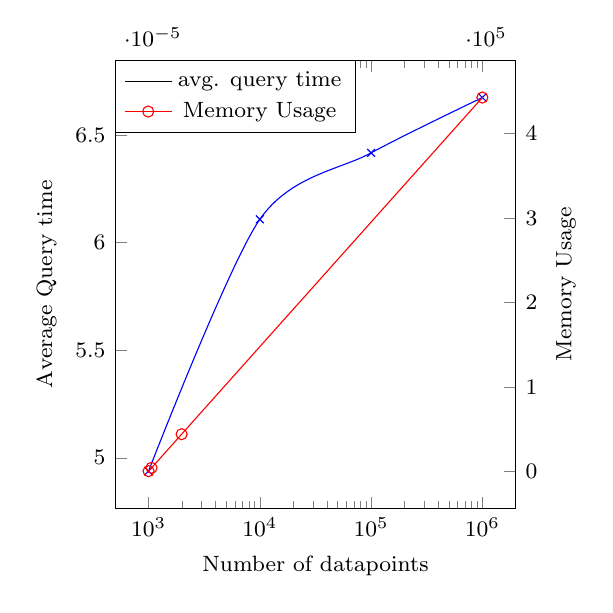
\begin{tikzpicture}
		\pgfplotsset{compat=1.10}
	\begin{axis}[
		legend style={at={(0,1)},anchor=north west},
		xmode=log,
		axis y line*=left,
		xlabel=Number of datapoints,
		ylabel=Average Query time,
		xtick={1000,10000,100000,1000000},
	]
	\addplot[smooth, mark=x, blue]
	coordinates{
		(1000, 4.93824E-05)
		(10000, 6.10835E-05)
		(100000, 6.41705E-05)
		(1000000, 6.67412E-05)
	}; \label{plot_one}
	\end{axis}
	
	\begin{axis}[
		legend style={at={(0,1)},anchor=north west},
  		axis y line*=right,
  		axis x line=none,
 	  	ylabel=Memory Usage,
	]
	\addlegendimage{/pgfplots/refstyle=plot_one}\addlegendentry{avg. query time}
	\addplot[smooth,mark=o,red]
  	coordinates{
    	(1000,444.0729167)
    	(10000.0148,4417.733333)
    	(100000.0295,44146)
    	(1000000.0441,442610.6667)
	}; \addlegendentry{Memory Usage}
	
\end{axis}	
\end{tikzpicture}
	\end{minipage}}
 \hfill 	
  \subfloat[Fully Connected Network]{
	\begin{minipage}[c][0.3\width]{
	   0.3\textwidth}
	   \centering
	   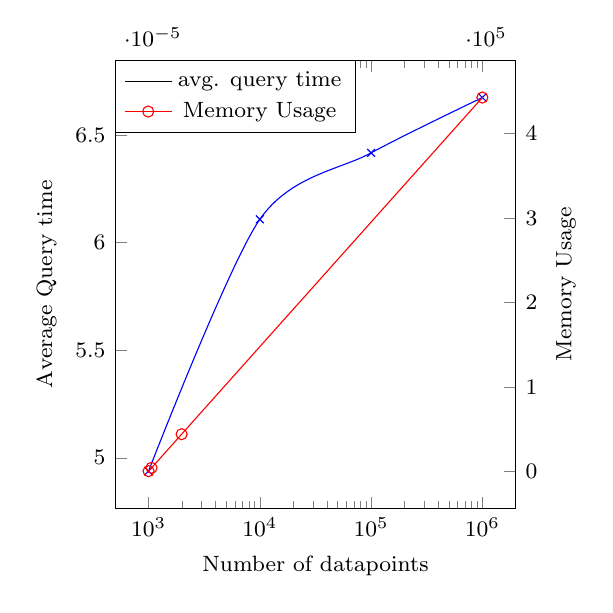
\begin{tikzpicture}
		\pgfplotsset{compat=1.10}
	\begin{axis}[
		legend style={at={(0,1)},anchor=north west},
		xmode=log,
		axis y line*=left,
		xlabel=Number of datapoints,
		ylabel=Average Query time,
		xtick={1000,10000,100000,1000000},
	]
	\addplot[smooth, mark=x, blue]
	coordinates{
		(1000, 4.93824E-05)
		(10000, 6.10835E-05)
		(100000, 6.41705E-05)
		(1000000, 6.67412E-05)
	}; \label{plot_one}
	\end{axis}
	
	\begin{axis}[
		legend style={at={(0,1)},anchor=north west},
  		axis y line*=right,
  		axis x line=none,
 	  	ylabel=Memory Usage,
	]
	\addlegendimage{/pgfplots/refstyle=plot_one}\addlegendentry{avg. query time}
	\addplot[smooth,mark=o,red]
  	coordinates{
    	(1000,444.0729167)
    	(10000.0148,4417.733333)
    	(100000.0295,44146)
    	(1000000.0441,442610.6667)
	}; \addlegendentry{Memory Usage}
	
\end{axis}	
\end{tikzpicture}
	\end{minipage}}
\caption{}
\end{figure}
\caption{blablabla}
\label{fig:whatever}
\end{figure}

	
0.000136657	28.515625
0.000119728	28.515625
0.00011154	28.515625
0.000137276	28.63541667
	
0.000279265	4666.032118
0.000272018	21933.81598
0.000255443	15421.51737
0.000325924	16624.75696

\textbf{Large Lognormal Distributed Data} The last dataset that we used is a large dataset that contains 190 million key value pairs that are distributed under lognormal distribution.